\section{Implementation – Sprint 1}

\subsection{Setting up an online repository (github, bitbucket, etc) for version control.}

We have set up a repository at: \href{https://github.com/hoangvvo/CO3001-SmartStudentPrintingService}{Git hub repository}
\subsection{Adding documents, materials and folders for Requirement, System modelling and Architectural design.}
Documents, materials, and folders for requirement, system modeling and architecture design have been added to the `docs` folder.
\begin{figure}[H]
    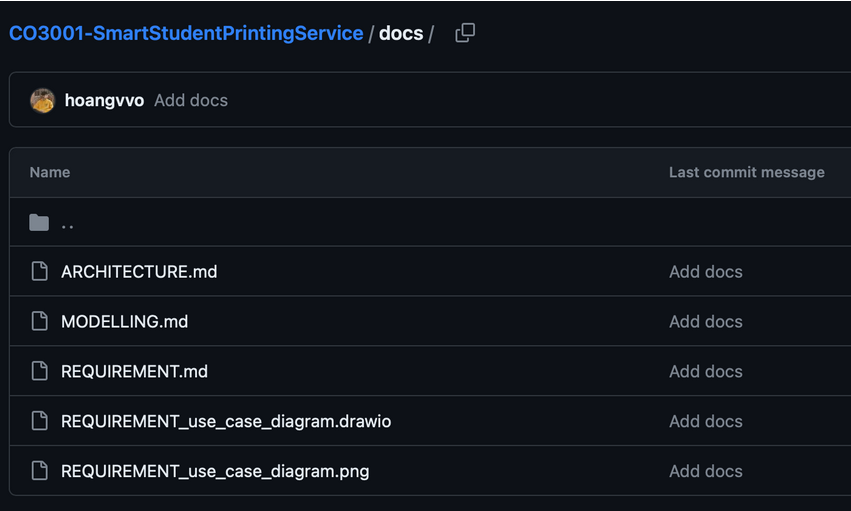
\includegraphics[max width = 0.9\linewidth,origin = c]{chapters/7. Implementation – Sprint 1/document,vv.png}
    \caption{Repository}%
\end{figure}

\subsection{Conducted a usability test with the user interface you developed in MVP 1.}
The following questions are used in the questionnaire to conduct the usability test. The test is performed online using Google Form.\\
The form can be found here: \href{https://forms.gle/c92x9Q3QJvYeMsRH6}{Google Form}
\subsubsection{Questions}
\textit{Basic questions:}
\begin{enumerate}
    \item Bạn đang học tập/công tác ở đâu?
    \item Bạn đang là sinh viên năm mấy?
    \item Bạn là sinh viên khoa…
\end{enumerate}
\indent \indent The reason for the basic questions is to understand the demography of the surveyees.\\
\indent \textit{Feedback questions:}\\
\indent \indent We are testing against the following features: Dashboard, Upload function, Print History, and Printer List.\\
\indent \indent For each page, we ask a series of grid multiple choice questions:
\begin{enumerate}
    \item Dễ sử dụng
    \item Thiết kế và thẩm mỹ
    \item Đáp ứng đầy đủ yêu cầu
\end{enumerate}
\indent \indent Each question can be answered from 1 (Strongly disagreed) to 5 (Strongly agreed).
\subsubsection{Responses}
The responses are collected in this Google Sheet: \href{https://docs.google.com/spreadsheets/d/19ywJ2WqR-1UwOe_dwIv6s4Ub5834-oyfKyqbfBqh974/edit#gid=1365939538}{Google Sheet}\\
\indent Here's a breakdown of the average ratings for each component of the application, considering the three aspects: Ease of Use, Design and Aesthetics, and Fulfillment of Requirements.\\
\indent Dashboard
\begin{itemize}[label =$\bullet$]
    \item \textbf{Ease of Use:} Average rating of about 3.02, indicating a moderate level of user-friendliness.
    \item \textbf{Design and Aesthetics:} Slightly lower rating of approximately 2.93, suggesting that the design might need improvements for better appeal.
    \item \textbf{Fulfillment of Requirements:} Average rating of around 3.07, showing that it moderately meets user needs.
\end{itemize}
\indent \indent Upload function
\begin{itemize}[label =$\bullet$]
    \item \textbf{Ease of Use:} Slightly higher average rating of approximately 3.09, indicating it's relatively user-friendly.
    \item \textbf{Design and Aesthetics:} Similar rating of about 3.07, suggesting an average design quality.
    \item \textbf{Fulfillment of Requirements:} A rating of around 3.12, which is slightly better, indicating it meets user needs well.
\end{itemize}
\indent \indent Print history
\begin{itemize}[label =$\bullet$]
    \item \textbf{Ease of Use:} A higher rating of around 3.16, suggesting good user-friendliness.
    \item \textbf{Design and Aesthetics:} Also higher, at about 3.12, indicating a more favorable design.
    \item \textbf{Fulfillment of Requirements:} Similar rating of approximately 3.09, showing it meets user needs adequately.
\end{itemize}
\indent \indent Printer List
\begin{itemize}[label =$\bullet$]
    \item \textbf{Ease of Use:} Average rating of about 3.07, indicating moderate ease of use.
    \item \textbf{Design and Aesthetics:} A bit lower at around 2.98, suggesting the design could be improved.
    \item \textbf{Fulfillment of Requirements:} An average rating of 3.0, indicating it meets user needs to a moderate extent.
\end{itemize}
\subsubsection{Conclusion}
In summary, the Print History component seems to be performing the best overall, with relatively higher ratings in all aspects. The Dashboard and Printer List components have lower ratings in design, which could be an area for improvement. The Upload function scores well in fulfilling user requirements, but its ease of use and design are average.

